\documentclass{article}

% if you need to pass options to natbib, use, e.g.:
\PassOptionsToPackage{numbers, compress}{natbib}
% before loading nips_2017
%
% to avoid loading the natbib package, add option nonatbib:
% \usepackage[nonatbib]{nips_2017}

\usepackage{nips_2018}

% to compile a camera-ready version, add the [final] option, e.g.:
% \usepackage[final]{nips_2017}

\usepackage[utf8]{inputenc} % allow utf-8 input
\usepackage[T1]{fontenc}    % use 8-bit T1 fonts
\usepackage{hyperref}       % hyperlinks
\usepackage{url}            % simple URL typesetting
\usepackage{booktabs}       % professional-quality tables
\usepackage{amsfonts}       % blackboard math symbols
\usepackage{nicefrac}       % compact symbols for 1/2, etc.
\usepackage{microtype}      % microtypography

\usepackage{hyperref}

\usepackage{amssymb}
\usepackage{amsmath}

% For citations
\usepackage{natbib}

% For figures
\usepackage{graphicx} % more modern
\usepackage{wrapfig}
%\usepackage{epsfig} % less modern
\usepackage{subfigure} 
\usepackage{multirow}
\usepackage{adjustbox}

\usepackage{listings}
\usepackage{textcomp}

% For assumptions
\usepackage{amsthm,amssymb,amsopn}
\newtheorem{assumption}{Assumption}
\newtheorem{define}{Definition}
\newtheorem{thm}{Theorem}
\newtheorem{lem}{Lemma}
\newtheorem{coro}{Corollary}
\newtheorem{condition}{Condition}
\usepackage{xspace}

% For algorithms
\usepackage{algorithm}
\usepackage{algorithmic}
\renewcommand{\algorithmiccomment}[1]{~~~~\textcolor{gray}{$\triangleright$\textit{#1}}}
\renewcommand{\algorithmicrequire}{\textbf{Input:}}
\renewcommand{\algorithmicensure}{\textbf{Output:}}
\makeatletter
\makeatletter
\newcommand*{\da@rightarrow}{\mathchar"0\hexnumber@\symAMSa 4B }
\newcommand*{\da@leftarrow}{\mathchar"0\hexnumber@\symAMSa 4C }
\newcommand*{\xdashrightarrow}[2][]{%
  \mathrel{%
    \mathpalette{\da@xarrow{#1}{#2}{}\da@rightarrow{\,}{}}{}%
  }%
}
\newcommand{\xdashleftarrow}[2][]{%
  \mathrel{%
    \mathpalette{\da@xarrow{#1}{#2}\da@leftarrow{}{}{\,}}{}%
  }%
}
\newcommand*{\da@xarrow}[7]{%
  % #1: below
  % #2: above
  % #3: arrow left
  % #4: arrow right
  % #5: space left 
  % #6: space right
  % #7: math style 
  \sbox0{$\ifx#7\scriptstyle\scriptscriptstyle\else\scriptstyle\fi#5#1#6\m@th$}%
  \sbox2{$\ifx#7\scriptstyle\scriptscriptstyle\else\scriptstyle\fi#5#2#6\m@th$}%
  \sbox4{$#7\dabar@\m@th$}%
  \dimen@=\wd0 %
  \ifdim\wd2 >\dimen@
    \dimen@=\wd2 %   
  \fi
  \count@=2 %
  \def\da@bars{\dabar@\dabar@}%
  \@whiledim\count@\wd4<\dimen@\do{%
    \advance\count@\@ne
    \expandafter\def\expandafter\da@bars\expandafter{%
      \da@bars
      \dabar@ 
    }%
  }%  
  \mathrel{#3}%
  \mathrel{%   
    \mathop{\da@bars}\limits
    \ifx\\#1\\%
    \else
      _{\copy0}%
    \fi
    \ifx\\#2\\%
    \else
      ^{\copy2}%
    \fi
  }%   
  \mathrel{#4}%
}
\makeatother

% for striking out.
\usepackage[normalem]{ulem}

% for todos
\usepackage{xargs}                      % Use more than one optional parameter in a new commands
\usepackage[pdftex,dvipsnames]{xcolor}
%todos -- remove at end
\usepackage[colorinlistoftodos,prependcaption,textsize=tiny]{todonotes}
\newcommand{\unsure}[2][1=]{\todo[linecolor=red,backgroundcolor=red!25,bordercolor=red,#1]{#2}}
\newcommand{\change}[2][1=]{\todo[linecolor=blue,backgroundcolor=blue!25,bordercolor=blue,#1]{#2}}
\newcommand{\info}[2][1=]{\todo[linecolor=OliveGreen,backgroundcolor=OliveGreen!25,bordercolor=OliveGreen,#1]{#2}}
\newcommand{\improvement}[2][1=]{\todo[linecolor=Plum,backgroundcolor=Plum!25,bordercolor=Plum,#1]{#2}}

% quick-and-dirty TKTKTK
\newcommand{\highlight}[1]{\colorbox{yellow}{#1}}

\newcommand{\ourModel}{EPPM\xspace}
\newcommand{\ourModelIR}{EPPM-IR\xspace}
\newcommand{\ourModelR}{EPPM-R\xspace}

\title{Predicting Electron Paths}

% The \author macro works with any number of authors. There are two
% commands used to separate the names and addresses of multiple
% authors: \And and \AND.
%
% Using \And between authors leaves it to LaTeX to determine where to
% break the lines. Using \AND forces a line break at that point. So,
% if LaTeX puts 3 of 4 authors names on the first line, and the last
% on the second line, try using \AND instead of \And before the third
% author name.

\author{
  David S.~Hippocampus\thanks{Use footnote for providing further
    information about author (webpage, alternative
    address)---\emph{not} for acknowledging funding agencies.} \\
  Department of Computer Science\\
  Cranberry-Lemon University\\
  Pittsburgh, PA 15213 \\
  \texttt{hippo@cs.cranberry-lemon.edu} \\
  %% examples of more authors
  %% \And
  %% Coauthor \\
  %% Affiliation \\
  %% Address \\
  %% \texttt{email} \\
  %% \AND
  %% Coauthor \\
  %% Affiliation \\
  %% Address \\
  %% \texttt{email} \\
  %% \And
  %% Coauthor \\
  %% Affiliation \\
  %% Address \\
  %% \texttt{email} \\
  %% \And
  %% Coauthor \\
  %% Affiliation \\
  %% Address \\
  %% \texttt{email} \\
}

\newcommand{\xb}{\mathbf{x}}
\newcommand{\Xc}{\mathcal{X}}
\newcommand{\Zc}{{\mathcal{Z}}}
\newcommand{\Mc}{{\mathcal{M}}}
\newcommand{\Bc}{{\mathcal{B}}}
\newcommand{\Ac}{{\mathcal{A}}}
\newcommand{\Pc}{{\mathcal{P}}}
\newcommand{\bb}{{\mathbf{b}}}
\newcommand{\ab}{{\mathbf{a}}}
\newcommand{\mb}{{\mathbf{m}}}
\newcommand{\Mb}{{\mathbf{M}}}
\newcommand{\Pb}{{\mathbf{P}}}
\newcommand{\Hb}{{\mathbf{H}}}
\newcommand{\Ab}{{\mathbf{A}}}
\newcommand{\Rc}{{\mathcal{R}}}
\newcommand{\delb}{{\boldmath{\delta}}}


%
\newcommand{\nodeEmbeddings}[1]{\Hb_{#1}}
\newcommand{\graphEmbeddings}{\mathbf{h_g}}
%\newcommand{\graph}{\mathcal{G}}



\newcommand{\actionLogits}{\textbf{s}} % for nodes

% The model definitions
\newcommand{\electronPath}{\Pc}
\newcommand{\moleculeSet}{\Mc}
\newcommand{\initialAndReactants}{\Mc_0, \Mc_r}

\newcommand{\contextVect}{\bm{c}}
% Then the modules!
\newcommand{\fEmbed}{g_{\Ac}} % for nodes
\newcommand{\fEmbedGraphs}{r} % for nodes


\newcommand{\fAdd}{f_{\textrm{add}}}
\newcommand{\fRemove}{f_{\textrm{remove}}}
\newcommand{\fInitial}{f_{\textrm{initial}}}
\newcommand{\fStop}{f_{\textrm{stop}}}
\newcommand{\fReagEmbed}{f_{\textrm{reagent}}}
\newcommand{\fModules}{\fEmbed, \fAdd, \fRemove, \fInitial,\fStop, \fReagEmbed}
\newcommand{\fui}{f_i}
\newcommand{\fuj}{f_j}
\newcommand{\fuk}{f_k}
\newcommand{\fum}{f_m}

\newcommand{\actionProb}[2][]{ p(a_{#2} \mid \moleculeSet_{\electronPath_{0:#2-1}^{#1}}, a^{#1}_{#2-1}, #2)}
\newcommand{\continueProb}[2]{p(s_{#1}' \mid \moleculeSet_{#2}) }

\begin{document}
% \nipsfinalcopy is no longer used

\maketitle

\begin{abstract}
The vast majority of chemical reactions can be described as the movement of pairs of electrons through a set of reactant molecules. 
As such, reactions are often described using `arrow-pushing' diagrams which show this movement as a sequence of arrows. 
We propose ElectroNet to learn these sequences directly from data.
Instead of predicting product molecules directly from reactant molecules in one-shot, learning a model of electron movement has the benefits of 
(a) being easy for chemists to interpret, 
(b) being able to incorporate the constraints of chemistry such as balanced atom counts each side, and 
(c) naturally encoding the sparsity of chemical reactions, which usually involve only a small number of atoms in the reactants.
Furthermore, we show that the model recovers basic knowledge of chemistry without being explicitly trained so.
% also it means the sides balance
\end{abstract}


\section{Introduction}

The ability to reliably predict the outcome of chemical reactions is of tremendous importance for the well-being of humanity, providing molecules which serve as medicines and materials. 

Theoretically, all chemical reactions can be described by the stepwise redistribution of electrons in molecules. 
Chemical reactions can be modelled at different levels of abstraction. On the lowest level, quantum-mechanical simulations can be performed: Changes in electronic structure are calculated by approximately solving the Schrödinger equation, which is computationally expensive for most systems of interest. 
On the other end, chemical reactions can be treated as rules that ``rewrite'' reactant molecules to products. While rules can be brittle, they allow to organize chemical knowledge by grouping reactions by these rules.
To combine the advantages of generality and commonality, chemists use a simple but tremendously powerful model, which describes the stepwise electron shifts using sequences of arrows which indicate bond making and breaking.\cite{herges1994organizing}

Machine learning has been applied for quantum chemistry\cite{NIPS2012_4830,schutt2017schnet}, and to predict global rewriting \cite{coley2017prediction,jin2017predicting,neural-symbolic,schwaller2017found,wei2016neural,zhang2005structure}. 
Kayala et al. proposed a model which consisting of two learned learning-to-rank and scoring steps, which however relies complex hand-coded rules and expert-annotated datasets, which are usually very small.\cite{kayala2011learning,kayala2012reactionpredictor}

Here, we propose ElectroNet, the first end-to-end model to learn sequences of electron shifts directly from large, unannotated datasets \todo{wording not yet elegant here}.



\section{Background}
In this section we describe the types of reactions we consider in this paper, and how it relates to previous work on reaction prediction. We then describe recent related work on deep graph models that inspire our model in the following section.

\paragraph{Chemical reactions.}
%In reality, the structure of a molecule is due to how electrons on each atom are interacting with each other. 

%% Bond localization?
Molecules consist of a set of atoms that are arranged into a structure by a set of bonds. 
As such, molecules can be depicted as a graph structure, where each node is an atom and each edge is a bond, 
as shown in Figure (note the convention that vertices which do not explicitly specify the atom name are assumed to be carbon C atoms). 

Each single bond represents the fact that two electrons are shared between the atoms that the bond connects\footnote{The vast majority of bonds in molecules are like this (so-called \emph{covalent} bonds), 
although our model also accommodates ionic bonds 
(in which one atom completely borrows the electrons of another atom and the atoms become charged.}.

%Molecules are broken and built via reactions. 
Just as electrons describe the current structure of molecules, they also describe how molecules react with other molecules to produce new ones. 
All chemical reactions involve the movement of electrons along paths of atoms in a set of reactant molecules. 
This movement causes the formation and breaking of chemical bonds that changes the reactants into a new set of product molecules.\footnote{This movement happens because it allows the set of molecules to move to a lower (and thus more favorable) energy state.} 
In this work, we will consider reactions that satisfy the following assumptions:
% \begin{enumerate}
% \item are single-step, so-called \emph{elementary} reactions.
% \item involve a pair of electrons, so-called \emph{heterolytic} reactions.
% \item either start with electrons on single atom, or with the electrons in an existing bond.
% \end{enumerate}
\begin{assumption}
Reactions are single-step\todo{MS:i am not sure this is really needed}, so-called \emph{elementary} reactions.
\label{assume:elem}
\end{assumption}

\begin{assumption}
Reactions involve pairs of electrons moving, so-called \emph{heterolytic} reactions.
\label{assume:het}
\end{assumption}

\begin{assumption}
Reactions either start with electrons on single atom (called \emph{free electrons}), or with the electrons in an existing bond.
\label{assume:atom_bond}
\end{assumption}

These sorts of reactions describe 81\% of \emph{organic reactions}\cite{herges1994coarctate} (i.e., reactions involving Carbon atoms) that have a large number of applications from drug design to the invention of new materials\cite{segler2018planning}\footnote{Organic reactions that do not satisfy these assumptions are homolytic reactions, and concerted reactions.}. 
%For this reason organic reactions has been the focus of recent work in reaction prediction in machine learning \cite{jin2017predicting,schwaller2017found}. 
Note that reactions which are multi-step can be decomposed into multiple single-step reactions in order to satisfy Assumption~\ref{assume:elem}.


\paragraph{Reactions as single electron paths.}
If reactions satisfy the above assumptions, then a chemical reaction is the result of pairs of electrons moving in a \emph{single path} through the reactant atoms. Further, this electron path will alternately remove existing bonds in molecules, and form new ones. We show this alternating structure in two example single-path reactions in Figure~\ref{fig:example}. In Figure~\ref{fig:example}(a) the reaction starts with the electrons in a bond, and in Figure~\ref{fig:example}(b) the reaction starts with the electrons in an atom. 

There are a number of benefits of predicting electron paths over predicting the outcomes of reactions directly (as in previous work \cite{jin2017predicting,schwaller2017found}):
\begin{itemize}
\item \textbf{Easy to interpret}: If the model makes a mistake, it is easy to see where it goes wrong by comparing the steps of the path with the correct steps.
\item \textbf{Sparse}: Reactions often only affect between 3 and 7 atoms out of anywhere from 10-50 reactant atoms. Modeling the reaction as a path allows us to exploit this sparsity.
\item \textbf{Chemical constraints}: Learning a path allows us to easily incorporate chemical constraints, such as the alternating removal and addition of bonds, among others.
\item \textbf{Compositionality}: Learning to combine lower-level abstractions of chemistry potentially allows to generalize better.
\end{itemize}


\begin{figure*}
\centering
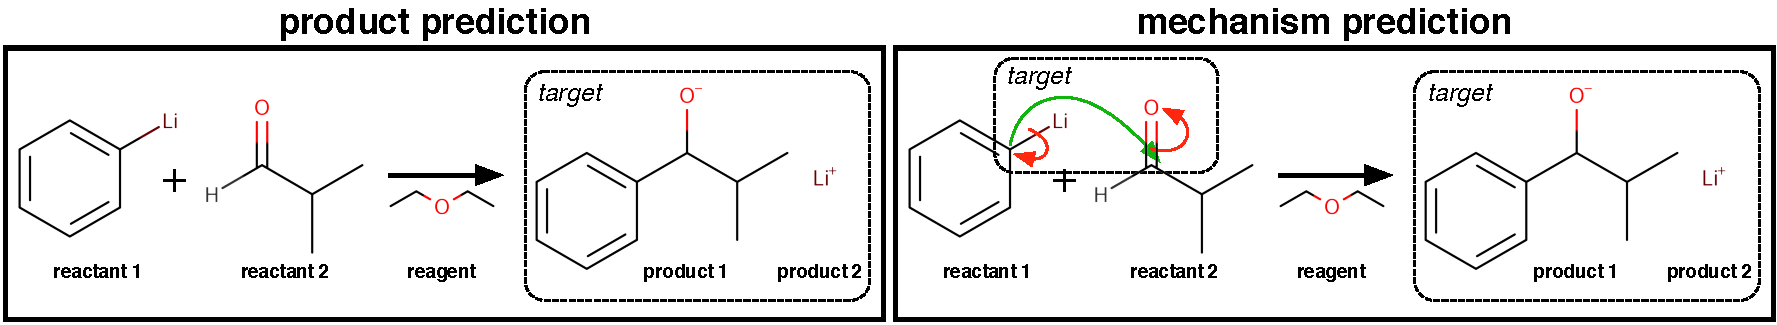
\includegraphics[width=\textwidth]{reaction_diagram}
\caption{reactions}
\end{figure*}

% KEY: separate assumptions from data processing
% !TEX root =  ../main.tex

\section{Model}



\begin{figure*}
\centering
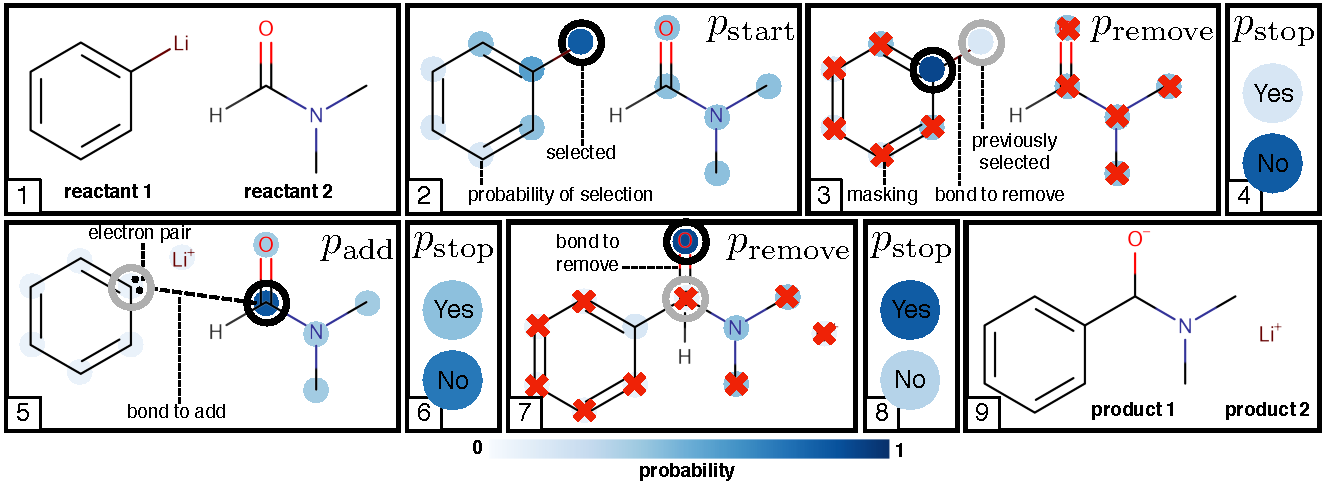
\includegraphics[width=\textwidth]{reaction_model_blue}
\caption{A visualization of the actions taken by the model to sequentially perform a simple reaction.}
\label{fig:reaction_model}
\end{figure*}



In this section we define a probabilistic model that describes the flow of movement of electrons that define an elementary heterolytic reaction.
We represent a set of molecules as a set of graphs $\moleculeSet$, with atoms $\Ac$ as vertices and bonds $\Bc$ as edges;
each connected component of the graph defines an individual molecule.
We can associate an ordering over all the atoms in all the molecules in the set using an {\em atom map} number,
an integer label assigned to each non-hydrogen atom in both the reactants and the products which 
both permits easy matching between atoms before and after the reaction, and
%\footnote{In the USPTO dataset, all reactions have been ``atom mapped'', which means that integer labels have been assigned to each non-hydrogen atom in both the reactants and the products.}. 
gives us a consistent way to index particular atoms.
Each atom $v \in \Ac$ includes a set of features, such as its atom type (e.g. carbon, oxygen, \dots); the full list of input atom features can be found in Table 1 of the supplementary material.
Input molecules into the model are first put in a Kekul\'e form, a process which makes explicit the location of single and double bonds in aromatic structures;
each bond $b \in \Bc$ is either a single, double, or triple bond.


Given an initial set of reactant molecules $\moleculeSet_0$ and a set of reagent molecules $\moleculeSet_r$, 
our model defines a conditional distribution over a sequence of atoms $\electronPath_{0:T} = (a_0, a_1, \ldots, a_T)$,
which fully characterizes the electron path.
\improvement[]{maybe instead $\electronPath$ goes up to $T-1$ and $\moleculeSet$ goes up to $T$? then both are length $T$}
This electron path in turn deterministically defines both a final product $\moleculeSet_{T+1}$, 
denoting the outcome of the reaction,
as well as a sequence of intermediate products $\moleculeSet_t$, for $t = 1,\dots,T$,
which correspond to the state of the graph after the first $t$ steps in the subsequence $\electronPath_{0:t} = (a_0, \dots, a_t)$ are applied to the initial $\moleculeSet_0$.


We propose to learn a parameterized distribution $p_\theta( \electronPath_{0:T} \mid \moleculeSet_0, \moleculeSet_r)$ over electron movements. 
We begin by describing the generative process %(i.e., the forward pass) 
of $p_\theta$, and then describe how to train the model parameters.


\subsection{Generative process}

The joint probability of an electron path can be factorized into a product of distributions
defining the probability $p(a_0 \mid \initialAndReactants)$ of the initial state $a_0$ given the reactants and reagents, 
the conditional probability $p(a_t \mid a_{t-1}, \moleculeSet_t, t)$ \todo[]{maybe somehow refer to "bond type" instead of $t$?} of next state $a_t$ given the intermediate products $\moleculeSet_t$ for $t > 0$,
and the probability $p(s_t \mid \moleculeSet_t)$ that the reaction terminates with final product $\moleculeSet_{t}$.

%The distribution over electron paths can be factorized as follows:
%%\begin{align}
%%p_\theta(\electronPath \mid \moleculeSet_0) = p_\theta(s_{0}' \mid \moleculeSet_0) p_\theta(a_{0} \mid \moleculeSet_0) \prod_{t=1}^{T-1} \left( p_\theta(a_{t} \mid a_{t-1}, \Mc_{t-1} ) p_\theta(s_{0}' \mid \moleculeSet_0) \right) p_\theta(a_{T} \mid a_{T}, \Mc_{T-1} ) p_\theta(s_{T} \mid \moleculeSet_T) \nonumber
%%\end{align}
%
%\begin{align*}
%p(\electronPath_{0:T} \mid \initialAndReactants) = &
% \quad 
% p(s_0' \mid \initialAndReactants)
% p(a_0 \mid \initialAndReactants)
% \prod_{t=1}^{T} \Big[ 
% 	p(s_t' \mid \initialAndReactants, \electronPath_{0:t-1})
% 	p(a_t \mid \initialAndReactants, \electronPath_{0:t-1} ) 
% \Big] \\
% & \times p(s_{T+1} \mid  \initialAndReactants, \electronPath_{0:T} )
%\end{align*}

%\improvement[]{this part a bit messy}
%Where $p(s_{t})$ is the probability of stopping the path before picking the $t^{\text{th}}$ action, $p(s_{t}')$ of continuing.


In practice we assume that the probability of an action depends only on (i) the intermediate molecule formed by the action path up to that point, (ii) the previous action taken (indicating where the free pair of electrons are) and (iii) the point of time through the path, indicating whether we are on an add or remove bond step. 
We further make the simplifying assumption that the stop probability and the actions after $a_0$ do not depend on the reagents. This leads to a parameterized model with dependency structure:
\begin{align}
\label{eq:jointprob}
p_\theta(\electronPath_{0:T} \mid \moleculeSet_0, \moleculeSet_r) 
&=
	p_\theta(s'_0 \mid \moleculeSet_0)
	p_\theta(a_0 \mid \moleculeSet_0, \moleculeSet_r)\\ \nonumber &\quad \times
	\left[\prod_{t=1}^{T}
		p_\theta(s_{t}' \mid \moleculeSet_{t})
		p_\theta(a_t \mid \moleculeSet_{t}, a_{t-1}, t)
	\right]
	p_\theta(s_{T+1} \mid \moleculeSet_{T+1})
	,
\end{align}
where we have defined $p(s'_t \mid \moleculeSet_t) \equiv 1 - p(s_t \mid \moleculeSet_t)$ to be the probability of {\em continuing} a reaction given the current molecule set $\moleculeSet_t$.
%
%
%%% THIS IS THE PREVIOUS VERSION:
%\begin{align*}
%p_\theta(\electronPath_{0:T} \mid \moleculeSet_0, \moleculeSet_r) = &
% \quad \continueProb{0}{0}
%       p(a_0 \mid \moleculeSet_0, \moleculeSet_r)
%       p(a_1 \mid \moleculeSet_0, a_0) \\
%       & \times \prod_{t=2}^{T} \Big[
%              \continueProb{t}{\electronPath_{0:t-1}}
%              \actionProb{t}
%       \Big] \\
%       & \times p(s_{T+1} \mid \moleculeSet_{\electronPath_{0:T}})
%\end{align*}
%
Note that you cannot stop after one action, as you have to pick up a complete electron pair;
however, it is possible to stop prior to selecting a first atom $a_0$, indicating that no reaction would take place.
Given any particular selected atom $a_t$ which extends the reaction path, we can deterministically update the previous molecular graph $\moleculeSet_{t}$ to produce the next set of (intermediate) products $\moleculeSet_{t+1}$.

If the three reaction assumptions stated in the previous section hold, then, as stated earlier, there are two types of electron movements that alternate: 
(1) movement that \emph{removes an existing bond}, and 
(2) movement that \emph{adds a new bond}. 
We can generalize assumption 3 by defining that atoms with free electrons have a self-bond. 
Thus, all reactions start by first selecting an atom, removing a bond (between two different atoms, or a self-bond), and then alternately adding and removing bond;
we can determine whether a particular step is an add step or remove step by inspecting $t$.
Note that $\moleculeSet_1 = \moleculeSet_0$, as the initial action of selecting $a_0$ does not remove or form any bonds\todo{maybe put this somewhere else}.

Each of the conditional probabilities in Eq.~\eqref{eq:jointprob} is parameterized by a neural network:
for each stage the network takes the current intermediate product graph, 
along with the previous action and the reagents if relevant, 
to compute a probability distribution over next possible actions (i.e., selecting a particular atom, or stopping).
These structure of these networks will be described in the following section and more detailed information on the architectures is given in the supplementary material.

Figure~\ref{fig:reaction_model} shows a simple example reaction, which demonstrates all the critical features of the model.
The first subfigure shows two reactants, which we assume will react (i.e.\ $s_0' = 1$).
Subsequent subfigures show the network picking an initial atom to begin the electron path,
and then iteratively selecting atoms for removing and adding bonds, potentially stopping after each action.
Masking at each add and remove step can reduce the total number of possibilities: 
for example, it is not possible to remove a bond which does not exist in the graph $\moleculeSet_t$.
\todo[]{walk through figure. do we want to that HERE, or in the caption? or elsewhere?}

\subsection{Computing atom and molecule features}


We are left now with defining the functional form of our conditional distributions for continuing $p_\theta(s'_t \mid \moleculeSet_t)$, picking the initial action $p_\theta(a_0 \mid \initialAndReactants)$, and picking subsequent actions $p_\theta(a_t \mid a_{t-1}, \moleculeSet_t, t)$.
However, before describing these modules we need to describe how we compute node embeddings and graph embeddings as these  are  essential to each.
Full architectural details (e.g.\ number of layers and hidden units) are deferred to the supplemental material.

Node embeddings are representations of all the atoms (vertices) in all the molecules present in $\moleculeSet_t$.
 We denote them by the matrix $\nodeEmbeddings{\moleculeSet_t} \subseteq \Rc^{|\Ac|\times d}$.
Each row contains a $d$-dimensional embedding of an atom (vertex).
A natural ordering for the rows are  the corresponding atoms' atom-mapped numbers.
We define the function $\fEmbed$ to take in a set of graphs representing each molecule and compute these node embeddings.
In general $\fEmbed$ could be any deep graph model that uses the graph structure of $\Mc_t$ to get graph-isomorphic node features, usually via message-passing techniques \citep{gilmer2017neural};
we choose to use gated graph neural network (GGNN) message functions \citep{li2016gated}.

It is also useful to be able to calculate graph embeddings $\graphEmbeddings$, which are vectors that represent groups of nodes belonging to one or more graphs; i.e.\ an entire molecule or set of molecules.
 We define the function that takes node features belonging to one or more graphs, and calculates their graph embedding by $\fEmbedGraphs$.
These are similar to the readout functions used for regressing on graphs detailed in \citep[Eq. 3]{gilmer2017neural} and the graph embeddings described in \citet[\S B.1]{li2018learning}. \todo[]{check ref the correct parts of these other papers.}
Specifically, $\fEmbedGraphs$ consists of three functions, $\fui$, $\fuj$ and $\fuk$, which could be any MLP but in practice we find that linear functions suffice. % use linear layers for.
There are two stages:
In stage (i), similar to \citet[\S B.1]{li2018learning} we form an embedding of one or more graphs (with vertices $\Ac'$), by performing a gated sum over the node features
\todo{BP: i added $\fuk$ to this equation, so it was all together --- hope this does not cause notational problems elsewhere}
\begin{align}
	\graphEmbeddings = \fuk\big(\sum_{v \in \Ac'} \left[ \mbox{sigmoid}(\fui(\Hb_{\Ac,v})) \cdot \fuj(\Hb_{\Ac,v}) \right]\big).
\end{align}

In this manner the function $\fui$ is used to decide how much that node should contribute towards the embedding,
 and $\fuj$ projects the node embedding up to a higher dimensional space; following \citet[\S B.1]{li2018learning}, we choose to be double the dimension of the node features.
Having formed this embedding of the graphs, we project this down to a lower dimensional space, which is done by the function $\fuk$. 
%Again we use a single linear layer for this function. % already said this above


\subsection{Computing our probabilities over actions}

Having described how we compute node and graph embeddings we are now ready to describe each of our action modules. We start with $p_\theta(s'_t \mid \moleculeSet_t)$, which is the probability of continuing given the set of intermediate products at time $t$. This probability is computed as a graph embedding down to one dimension followed by a sigmoid function: $p_\theta(s'_t \mid \moleculeSet_t) = \sigma(\fEmbedGraphs_{\textrm{stop}}(\nodeEmbeddings{\moleculeSet_t}))$.


This leaves us with describing the form of the initial action, $p_\theta(a_0 \mid \initialAndReactants)$, and picking subsequent actions, $p_\theta(a_t \mid a_{t-1} \moleculeSet_t, t)$, modules.
 The second of these can be broken down into two parameterized functions
$p_\theta^\textrm{remove}(a_t \mid a_{t-1}, \moleculeSet_t)$ for the remove bond step, taken when $t$ is odd, and $p_\theta^\textrm{add}(a_t \mid \moleculeSet_t, a_{t-1})$ for the add bond step, taken when $t$ is even. 
 Each of these three parameterized conditional probability distributions for the {\em initial}, {\em add} and {\em remove} steps have similar forms, and produce a probability vectors over actions as their output. 
 
 Each of these modules start by computing  a single value for each node, so for the initial step we have 
 $\actionLogits_{\textrm{initial}, v} = \fum^\textrm{intial}(\nodeEmbeddings{\moleculeSet_t,v}, \contextVect)$ where $\fum$ is a NN and $\contextVect$ is a context vector. The expressions are similar for the add and remove modules, however with different NNs used for the respective $\fum$ functions.
 Moreover, they also differ in the context vectors, $\contextVect$, which they use; for the add, $p_\theta^\textrm{add}(a_t \mid \moleculeSet_t, t)$, and remove steps, $p_\theta^\textrm{remove}(a_t \mid \moleculeSet_t, t)$, this context vector is the node embedding of the previous action, $\nodeEmbeddings{\moleculeSet_t, a_{t-1}}$. 
 For the initial step, this context vector $\contextVect$ if computed by summing the graph embeddings for each reagent, computed using the embedding function $\fEmbedGraphs_r$.

Finally, each of the modules compute the probability vector over actions. So again starting with the initial step we have 
$p_\theta(a_0 \mid \initialAndReactants) \propto \bm{\beta_\textrm{initial}} \odot \mbox{softmax}(\bm{\actionLogits_{\textrm{initial}}})$, 
with again similar terms for the add and remove steps.  
The $\bm{\beta}$ term is a binary vector, that allows us to mask out specific actions. The value of this differs for the {\em initial}, {\em add} and {\em remove} steps. 
For the initial step any action (or atom) can be picked and so this is 1 everywhere. For the remove step, $\bm{\beta_\textrm{remove}}$ masks out bonds that do not currently exist (although self bonds are allowed in the first step).
For the add step, $\bm{\beta_\textrm{add}}$ only masks out the previous action.



\paragraph{Training}
We can learn the parameters $\theta$ of all the parameterized functions, by maximizing the likelihood of the true path $\log p_\theta(\electronPath_{0:T} \mid \moleculeSet_0, \moleculeSet_r)$.
%\begin{align*}
%%  \min_{\fModules}
%\min_{\theta}
%    & - \log \continueProb{0}{0} - \log p(a_0 \mid \moleculeSet_0, \moleculeSet_r)  - \log p(a_1 \mid \moleculeSet_0, a^*_0) \\
%	& - \sum_{t=2}^{T} \log \Big[ \continueProb{t}{\electronPath_{0:t-1}^*} \actionProb[*]{t} \Big] \\
%    & - \log p(s_{T+1} \mid \moleculeSet_{\electronPath_{0:T}^*})
%\end{align*}
This is evaluated by using a known true electron path $a_t^\star$ and intermediate products $\moleculeSet_t^\star$ extracted from training data,
rather than on simulated values. 
This allows us to train on all stages of the reaction at once.

\paragraph{Sampling}
Once trained we can sample chemically-valid paths from our model using beam search.  This is procedure is described in \todo[]{briefly describe beam search}. 








 




% While this assigns probabilities to discrete actions this can be a function of continuous embeddings of molecules as above. 

% To learn $g_\theta$, one idea is to sample a path $\Pc$ and apply it to our initial set of molecules $\Mc_0$. Using the known deterministic function $f$ we can produce a final predicted set of molecules $\hat{\Mc}_T$. However, even if we have a loss function $\ell(\hat{\Mc}_T,\Mc_T)$ we cannot use REBAR or RELAX to compute $\frac{\partial \ell(\hat{\Mc}_T,\Mc_T)}{\partial \theta}$ because $f$ is not stochastic. Maybe it's possible to make $f$ stochastic, then maybe it is possible to apply REBAR or RELAX.

% Another idea is to learn $g_\theta$ via maximum likelihood. Specifically, $g_\theta$ assigns some probability to all possible paths, so we can adjust $\theta$ to make the paths that lead to $\Mc_T$ more likely and those that do not less likely. I believe an efficient way to do this is to roll out only a few paths to produce $\hat{\Mc}_T$ (i.e., using the valid path sampling method using Algorithm~\ref{algo:valid_path}) and then update $\theta$ via $\frac{\partial \ell(\hat{\Mc}_T,\Mc_T)}{\partial \theta}$. Maybe Monte Carlo Tree Search could be useful here? I need to read more about this. 

% \subsection{Notes}
% In general I haven't given as much thought to a stochastic model. This is because ultimately we don't really want to give a chemist a distribution over electron paths, they want to know an actual prediction of electron movements. One could argue that this distribution might be a proxy for reaction `energy', but I don't think we need to learn a distribution to get this. We could make Algorithm 1 stochastic by instead of selecting the closest atom in steps 6 and 12, we select an atom with Gaussian probability given by the Euclidean distance between atoms in $\Mc_t$ and the predicted action $\hat{\ab}$. It's not clear to me whether this is a better or worse proxy for reaction energy.

% The main question is whether it will be easier to learn a stochastic function or two deterministic functions that give realistic electron paths. I think this boils down to (a) can we sample enough roll-outs to get a peaky distribution, (b) will learning both $g$ and $f$ lead to too much approximation error.



% We propose to learn a function $g: \Mc \rightarrow \Pc$. 

% Because we do not know the true path $\Pc$, we can only receive a learning signal from the final predicted product molecules $\hat{\Mc}_T$ (compared to the true final molecules $\Mc_T$. This final predicted product is a deterministic (known) function $f$ of the initial molecules $\Mc_0$ and predicted actions $\hat{\Pc}$ (from $g$), as such $f(\Mc_0, \hat{\Pc}) = \hat{\Mc}_2, \ldots, \hat{\Mc}_T$.

% Ideally, we would like to learn the parameters of $g$, called $\theta$, to minimize the difference between the predicted final molecules $\hat{\Mc}_T$ and $\Mc_T$ (i.e., via some loss function $\ell$). However, we cannot resort to gradient-based techniques to learn $g$ because the inputs and outputs of $g$ are discrete objects, and the function $f$ producing $\hat{\Mc}_T$ is also discrete so the gradient $\frac{\partial \ell(\hat{\Mc}_T,\Mc_T)}{\partial \theta}$ does not exist. To solve this, we propose two types of models for this problem.

% \paragraph{Deterministic.}
% Instead, we assume we have continuous mappings from molecules $\Mc$ to vectors $\mb$ and paths $\Pc$ to matrices $\Pb$. We propose to learn continuous functions $g_\theta: \mb \rightarrow \Pb$ and $f_\phi: \mb, \Pb \rightarrow \mb, \ldots, \mb$. Then we can compute derivatives of a loss function $\ell(\hat{\mb}_T,\mb_T)$ with respect to parameters $\theta$ as follows. Let $\hat{\mb}_T = [f(\mb_1,g(\mb_1))]_T$. Then our gradient is $\frac{\partial \ell(\hat{\mb}_T,\mb_T)}{\partial \theta} = \frac{\partial \ell(\hat{\mb}_T,\mb_T)}{\partial f}\frac{\partial f}{\partial g}\frac{\partial g}{\partial \theta}$.

% Note that now, $f_\phi$ is unknown. So we propose to learn it given observed traces: $(\mb_1,\Pb,\mb_2,\ldots,\mb_T)$. For simplicity define $\Mb_{2:T} = [\mb_2,\ldots,\mb_T]$, and $f(\mb_1,\Pb) = \hat{\Mb}_{2:T}$. Then, given a loss function $l(\hat{\Mb}_{2:T},\Mb_{2:T})$ we can learn the parameters of $f$, called $\phi$ via the gradient $\frac{\partial l(\hat{\Mb}_{2:T},\Mb_{2:T})}{\partial \phi} = \frac{\partial l(\hat{\Mb}_{2:T},\Mb_{2:T})}{\partial f} \frac{\partial f}{\partial \phi}$.

% In order to ensure that $g_\theta$ produces paths $\hat{\Pb}$ that are valid (i.e., that alternately remove and add bonds) we propose to take a predicted path $\hat{\Pb}$ and map it to a valid path $\Pb^*$ as described in Algorithm~\ref{algo:valid_path}. Given a valid path, we propose a loss function $L(\hat{\Pb},\Pb^*)$ and learn $g_\theta$ to minimize this loss via $\frac{\partial L(\hat{\Pb},\Pb^*)}{\partial \theta} = \frac{\partial L(\hat{\Pb},\Pb^*)}{\partial g} \frac{\partial g}{\partial \theta}$.



% %another loss function 
% %Finally, one last appealing property of this model is that if similar molecules have similar continuous representations embeddings then the functions $g_\theta, f_\phi$ allow us to generalize to similar molecules we have not seen before.
% Function $f_\phi$ could be an RNN and $g_\theta$ could be a fully connected network. We could consider an alternative $g_\theta$ that is conditioned on previous states which could be an RNN. 



% \paragraph{Stochastic.}

%Given a learned distribution we could sample valid paths using Algorithm~\ref{algo:valid_path}. We could use a model similar to DRAW. Maybe it is possible to not learn $f$ and instead use a dynamic programming algorithm to update $g_\theta$. Otherwise, we could learn $f$ as a stochastic function over discrete states. In general I haven't given as much thought to a stochastic model.
%Note that this distribution is not Markov as we need to know if the previous two electron movement added or removed a bond, in order to determine whether we need to consider only existing bonds or not. We could use a model similar to DRAW and mask all samples so agree with these constraints.




% TODO:
% - write intuitive idea
% - formalize variables
% - wait a long time until writing objective
% - wait even longer to write optimization

\section{Experiments}

% describe USPTO dataset and preprocessing
% !TEX root =  ../main.tex

%\subsection{Data and preprocessing}

Our dataset for evaluating our model is a collection of chemical reactions extracted from the US patent database \citep{Lowe2017}.
We take as our starting point the 479,035 reactions, along with the training, validation, and testing splits 
which were used by \citet{jin2017predicting}, referred to as the USPTO dataset.
This data consists of, per reaction, a group of bond changes and reaction SMILES strings \citep{weininger1988smiles}.
The bond changes indicate pairs of atoms which are connected differently in the reactants and products.
The SMILES strings encode the molecules present in a text based format.
Before we can apply our method, we perform two data preprocessing tasks described in the subsections below
(using the open-source chemo-informatics software RDKit \citep{rdkit}).
These steps automatically
extract a subset of data appropriate for training our model of electron movement during a reaction. 


\subsection{Reactant and reagent separation}

Typically, reaction SMILES strings are split into three parts --- reactants, reagents, and products.

The reactant molecules are those which are consumed during the course of the chemical reaction to form the  product, 
while the {\em reagents} are any additional molecules which provide context under which the reaction occurs (for example, catalysts),
but do not explicitly take part in the reaction itself; we see this in the example in Figure~\ref{fig:task-overview}.

Unfortunately, the USPTO dataset as extracted does not differentiate between reagents and reactants.
We elect to preprocess the entire USPTO dataset by separating out the reagents from the reactants using the process outlined in \citet{schwaller2017found}, where we classify as a reagent any molecule for which either 
(i) none of its constituent atoms appear in the product, or 
(ii) the molecule appears in the product SMILES completely unchanged from the pre-reaction SMILES.
This allows us to properly model molecules which are included in the dataset but do not materially contribute to the reaction.

\subsection{Identifying reactions with linear electron topology}

To train our model, it is necessary to extract a ground-truth representation of the electron paths from the SMILES strings and bond changes.
Furthermore, not every reaction in the USPTO dataset has a linear electron topology; 
such reactions (for example, multi-step reactions and cycloadditions) will not have a single unique path through the atoms 
which describes the movement of the electrons.

The first step is to look at the bond changes present in a reaction. 
Each atom on the ends of the path will be involved in exactly one bond change;
the atoms in the middle will be involved in two. 
We can then line up bond change pairs so that neighboring pairs have one atom in common,
 with this ordering forming a path.
For instance, given the pairs "\texttt{11-13, 14-10, 10-13}" we form the unordered path "\texttt{14-10, 10-13, 13-11}".
If we are unable to form such a path, for instance due to two paths being present as a result of multiple reaction stages, then we discard the reaction.

For training our model we want to find the ordering of our path, so that we know in which direction the electrons flow.
To do this we examine the changes of the properties of the atoms at the two ends of our path. 
In particular, we look at changes in charge and attached implicit hydrogen counts. 
The gain of negative charge (or analogously the gain of hydrogen as H$^+$ ions without changing charge) indicates that electrons have arrived at this atom, 
implying that this is the end of the path; 
vice-versa for the start of the path.
However, sometimes the difference is not available in the USPTO data, as unfortunately only major products are recorded, and so details of what happens to some of the reactant molecules' atoms may be missing.
In these cases we fall back to using an element's {\em electronegativity} to estimate the direction of our path, with more electronegative atoms attracting electrons towards them and so being at the end of the path. 

The next step of filtering checks that the path alternates between add steps (+1) and remove steps (-1). 
This is done by analyzing and comparing the bond changes on the path in the reactant and product molecules. 
Reactions that involve greater than one change (for instance going from no bond between two atoms in the reactants to a double bond between the two in the products) can indicate multi-step 
reactions with identical paths, and so are discarded.
Finally, as a last sanity check, we use RDKit to produce all the intermediate and final products induced by our path acting on the reactants,
to confirm that the final product that is produced by our extracted electron path is consistent with the major product SMILES in the USPTO dataset.

The end result of this is extracted reaction paths for those entries in the USPTO dataset which 
correspond to reactions of linear topology.
This comprises $73\%$ of the dataset, containing 349,898 total reactions, of which 29,360 form the held-out test set.




% having created dataset describe how trained and detailed model architecture.
\subsection{Training}

For our experiments we train our \ourModel models on these extracted paths.
We consider two variants of {\ourModel}s, one as defined before which includes reagent information, called \ourModelR, and one which ignores the reagents when selecting the initial actions which we call \ourModelIR.
We train our models for ten epochs using ADAM \citep{kingma2014adam} and an initial learning rate of $1e-4$.
We train on reaction minibatch sizes of one, although these can consist of multiple intermediate graphs.
For the GGNN we use four propagation steps and have input, node output and hidden layers all of size 101. 
The NNs representing $\fAdd$ and  $\fRemove$ consist of one hidden layer of dimension 100. 
The NN for $\fInitial$ has two hidden layers of size 100 for the \ourModelR when including reagent information and one hidden layer of size 100 when ignoring it in the \ourModelIR. In general we found architecture changes such as increasing a network by one or two hidden layers had less effect that including reagent information.
Further architecture and training details can be found in the supplementary material.

% describe issues with evaluation, results tables
% !TEX root =  ../main.tex

\subsection{Results and Evaluation}

Having trained our model, one surprising challenge is accurately defining what it means for our model to ``correctly'' predict the reaction outcome. 
Part of this relates to whether we are interested in  \emph{Reaction Mechanism Prediction} or \emph{Reaction Product Prediction}. \todo{these should have been described by now using fig 1 but back check.} 
In this section we evaluate our model in each of these regimes in turn.
%Sampling from our model, or selecting high-probability candidates using beam search, yields

\subsubsection*{Reaction Mechanism Prediction}

 For Reaction Mechanism Prediction we are interested in making sure that we got the exact sequence of actions correct.
For instance, when forming a bond between two pairs of atoms we want to know which one of the atoms donated the electron pair needed to form the bond, even if the end result is the same. 

The representation of the reaction mechanism produced by our model is a sequence of atoms, detailing the path taken by the electrons in a series of alternating steps in which bonds are broken and formed; this then can take the form of a sequence of integers.
Here in order to associate a fixed identity with each atom, these integers represent the ``atom mapped'' labels\footnote{In the USPTO dataset, all reactions have been ``atom mapped'', which means that integer labels have been assigned to each non-hydrogen atom in both the reactants and the products.} associated to each atom in the sequence.

The most straightforward approach then to evaluate our accuracy at predicting reaction mechanisms is to check whether the sequence of integers extracted from the raw data (by comparing the reported major product with the reactants\todo[]{change bracket content to "as described earlier"...?}) is an exact match with the sequence of integers output by our \ourModel; the top-1, top-2, top-3, and top-5 accuracies evaluated in this manner are reported in Table \ref{table:mech-predict}.

\begin{table}[h]
  \caption{Results when using \ourModel  for Reaction Mechanism Prediction. Here we count a prediction as correct if the atom mapped action sequences predicted by our model match exactly those extracted from the USPTO dataset.}
  \label{table:mech-predict}
  \centering
  \begin{tabular}{lllll}
    \toprule
    & \multicolumn{4}{c}{Accuracies (\%)}                   \\
    \cmidrule(r){2-5}
    Model Name & Top-1 & Top-2 & Top-3 & Top-5 \\
    \midrule
    \ourModelIR &  70.3 &  82.8 & 87.7 & 92.2    \\
    \ourModelR  &  77.8 &  89.2 & 92.4 & 94.7    \\
    \bottomrule
  \end{tabular}
\end{table}




\subsubsection*{Reaction Product Prediction}

Reaction Mechanism Prediction is useful for ensuring that we formed the correct product in the {\em correct way}.
However, this can underestimate the actual predictive accuracy of the model: 
although a single atom mapping is provided as part of the USPTO dataset, in general atom mappings are not unique; 
when a reactant contains some symmetries, then multiple different atom mappings are effectively equivalent.
Here this would manifest as multiple different sequences of integers which correspond to chemically identical electron paths. An example of a reaction falling under this category is given in the supplementary material.
\sout{An extreme example is a reaction in which one reactant is benzene, a molecule which is formed of six carbon atoms in a completely symmetric ring: while this would be present with a unique atom mapping in the dataset, any reaction path which includes one of these carbon atoms could equally well have selected any of the other five \todo{maybe toss in an inline figure with an example}.}

Recent machine learning approaches to Reaction Product Prediction \citep{jin2017predicting,schwaller2017found}
have evaluated whether the major product reported in the test dataset matches predicted candidate products generated by their system, independent of mechanism.
In our case, the top-5 accuracy for a particular reaction may include multiple different electron paths that ultimately yield the same product molecule.

Identifying whether two product molecules are chemically the same is equivalent to solving a graph isomorphism over the atoms and bond types, comparing the output of our system to the product molecule.
To perform this comparison, we consider an electron path as a sequence of edits performed on the reactants graph, apply these edits to define a product graph, 
and then define a deterministic mapping from the edited graph to a canonical string representation.
This is done by first Kekulizing the molecule, a process which makes explicit the location of single and double bonds in aromatic structures.
We then apply the sequence of edits to the reactants graph,
set explicit charges or hydrogen counts on the first and last atom in the electron path in order to satisfy valence constraints,
and strip all atom map numbers from the graph.
If this graph corresponds to a valid product molecule, we can then use RDKit to express the molecule in a canonical SMILES string format;
predicted electron paths which would yield chemically infeasible products are represented as an empty string.
We can then evaluate whether a predicted electron path matches the ground truth electron path by a string comparison.

To use our model to produce a ranked list of predicted products, we can compute the estimated canonicalized product SMILES for each of the outputs of our beam search over electron paths, removing duplicates along the way. 
These product-level accuracies are reported in \highlight{ROW OF TABLE}.

A benefit of our approach, even if the ultimate the desired goal is to predict the product molecule rather than the electron path,
is that the predicted electron paths then can serve as explanation.
For each predicted product molecule, there is at least one electron path generated by our model which produced this;
whichever of these was highest-ranked by the beam search corresponds to the maximum likelihood path, 
but we can also report the other candidate paths which would produce the sample output as alternative explanations.
\highlight{MAYBE EXAMPLE IN APPENDIX FIGURE.}





% !TEX root =  ../main.tex

\begin{figure*}[t]

    \centering
    \begin{subfigure}[b]{0.3\textwidth}
        \centering
        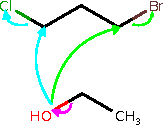
\includegraphics[height=0.9in]{imgs/textbook/reaction3}\\\vspace{0.1in}
        %\caption{}
    \end{subfigure}%
    \hspace{1cm}
     \begin{subfigure}[b]{0.5\textwidth}
        \centering
        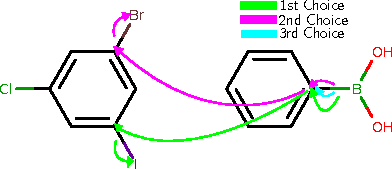
\includegraphics[height=1.1in]{imgs/textbook/reaction7}
        %\caption{}
    \end{subfigure}
%    \vspace{-1em}
	\caption{(Left) 2nd-order nucleophilic substitutions $S_N 2$-reactions, (right) Suzuki-coupling (please note that in the ``real'' mechanism of the Suzuki coupling, the reaction would proceed via oxidative insertion, transmetallation and reductive elimination at a Palladium catalyst. As these mechanistic details are unavailable, we treat Palladium as a reagent). 
    In both cases, our model has correctly picked up the trend that halides lower in the period table usually react preferably ($I>Br>Cl$). }
	\label{fig:qualitative}
\vspace{-0.5em}
\end{figure*}



\subsection{Qualitative Analysis}

Complex molecules often feature several potentially reactive functional groups $\mathcal{F}=\{F_1,...,F_N\}$, which compete for reaction partners. 
To predict the selectivity, that is which functional group will predominantly react in the presence of other groups, 
students of chemistry learn heuristics and trends, 
which have been established over the course of three centuries of experimental observation.
To qualitatively study whether the model has learned such trends from data we queried the model with several typical text book examples from the chemical curriculum (see Figure \ref{fig:qualitative} and the appendix). 
We found that the model predicts most examples correctly. In the few incorrect cases, interpreting the model's output reveals that the model made chemically plausible predictions.



\section{Discussion}



\bibliography{bibliography}
\bibliographystyle{plainnat}



<<<<<<< HEAD
%\begin{figure*}
%\centering
%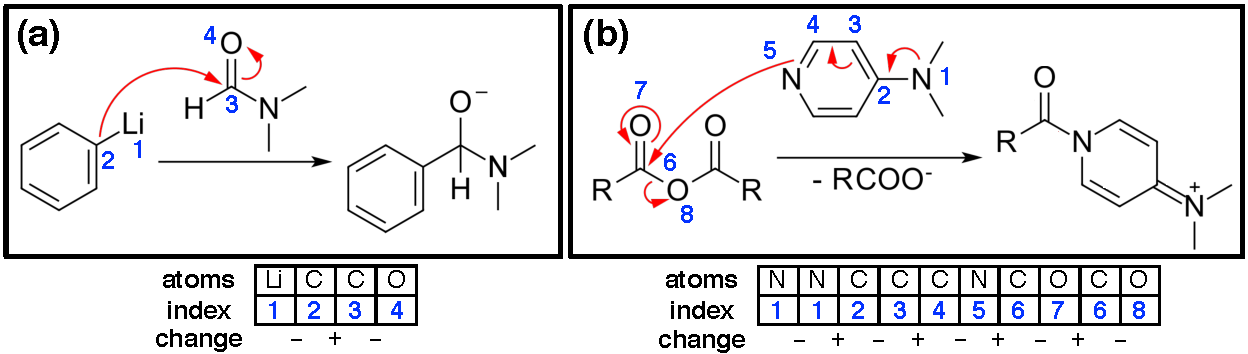
\includegraphics[width=\textwidth]{rxn_example}
%\vspace{-3ex}
%\caption{Two example reactions and their electron paths. In reaction (a), the reaction starts from an existing bond between Lithium (atom 1) and Carbon (atom 2). In reaction (b) the reaction starts from a lone-pair of electrons on Nitrogen (atom 1), which we represent formally as a bond with itself.}
%\label{fig:example}
%\end{figure*}
=======
% \begin{figure*}
% \centering
% 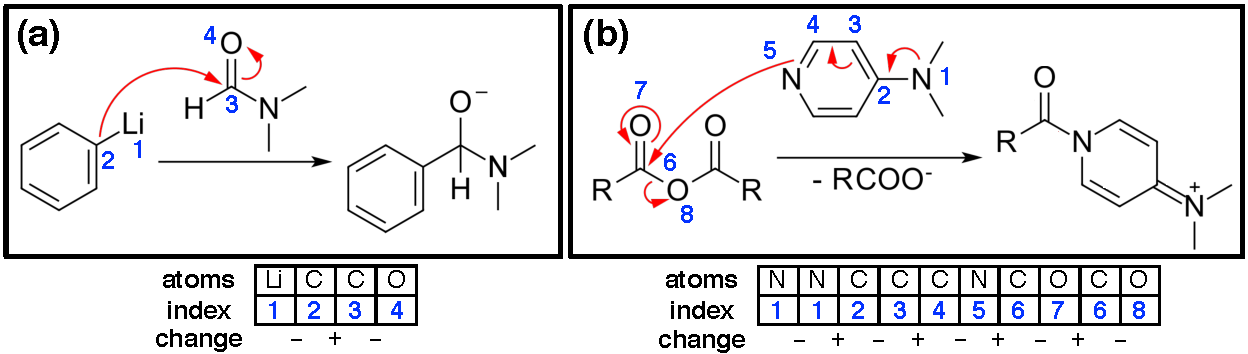
\includegraphics[width=\textwidth]{rxn_example}
% \vspace{-3ex}
% \caption{Two example reactions and their electron paths. In reaction (a), the reaction starts from an existing bond between Lithium (atom 1) and Carbon (atom 2). In reaction (b) the reaction starts from a lone-pair of electrons on Nitrogen (atom 1), which we represent formally as a bond with itself.}
% \label{fig:example}
% \end{figure*}
>>>>>>> 42256e04c3a064d70e6309a4cd8fa1d77f7acbdf


\end{document}
